\newpage\subsection*{Άσκηση 6}

\begin{enumerate}
        
\item[\textbf{\en{i.}}] Το  πρόβλημα  3 - 33  χωρίς  την  προσομοίωση.
\item[\textbf{\en{ii.}}] Το πρόβλημα 3 - 34 χωρίς το πρόγραμμα δοκιμαστικής εισόδου.
\item[\textbf{\en{iii.}}] Το πρόβλημα 3 - 36. 

\end{enumerate}

\subsubsection*{Λύση}

\begin{enumerate}
\item[\textbf{\en{ia.}}]
\selectlanguage{english}
\begin{center}
    \begin{tabularx}{0.95\textwidth}[t]{|Y|Y|Y|Y|Y|Y|Y|Y|}
\hline 
ns & x & y & x' & y' & x\&y' & y\&x' & xor \\ 
\hline 
-1 & 0 & 0 & 1 & 1 & 0 & 0 & 0 \\ 
\hline 
0 & 0 & 1 & 1 & 1 & 0 & 0 & 0 \\ 
\hline 
2 & 0 & 1 & 1 & 1 & 0 & 0 & 0 \\ 
\hline 
4 & 0 & 1 & 1 & 0 & 0 & 0 & 0 \\ 
\hline 
6 & 0 & 1 & 1 & 0 & 0 & 0 & 0 \\ 
\hline 
8 & 0 & 1 & 1 & 0 & 0 & 1 & 0 \\ 
\hline 
10 & 0 & 1 & 1 & 0 & 0 & 1 & 0 \\ 
\hline 
12 & 0 & 1 & 1 & 0 & 0 & 1 & 0 \\ 
\hline 
14 & 0 & 1 & 1 & 0 & 0 & 1 & 0 \\ 
\hline 
16 & 0 & 1 & 1 & 0 & 0 & 1 & 0 \\ 
\hline 
18 & 0 & 1 & 1 & 0 & 0 & 1 & 1 \\ 
\hline 
20 & 0 & 1 & 1 & 0 & 0 & 1 & 1 \\ 
\hline 
22 & 0 & 1 & 1 & 0 & 0 & 1 & 1 \\ 
\hline 
50 & 0 & 1 & 1 & 0 & 0 & 1 & 1 \\ 
\hline 
\end{tabularx} 
\end{center}
\selectlanguage{greek}

\hfill

\item[\textbf{\en{ib.}}]
\selectlanguage{english}
\inputminted{verilog}{askisi6i.v}
\selectlanguage{greek}

\hfill
\item[\textbf{\en{ii.}}]
\selectlanguage{english}
\inputminted{verilog}{askisi6ii.v}
\selectlanguage{greek}

\newpage
\item[\textbf{\en{iiia.}}]
\hfill
\begin{center}
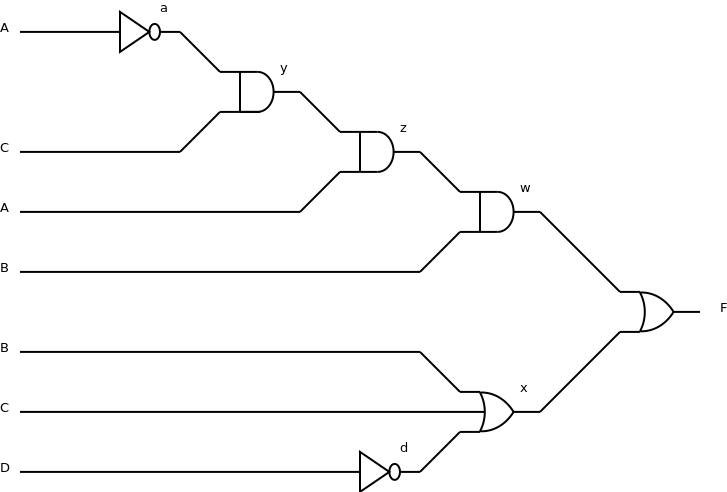
\includegraphics[width=.5\textwidth, center]{Diagram2.png}
\end{center}

\hfill
\item[\textbf{\en{iiib.}}]
\hfill
\begin{center}
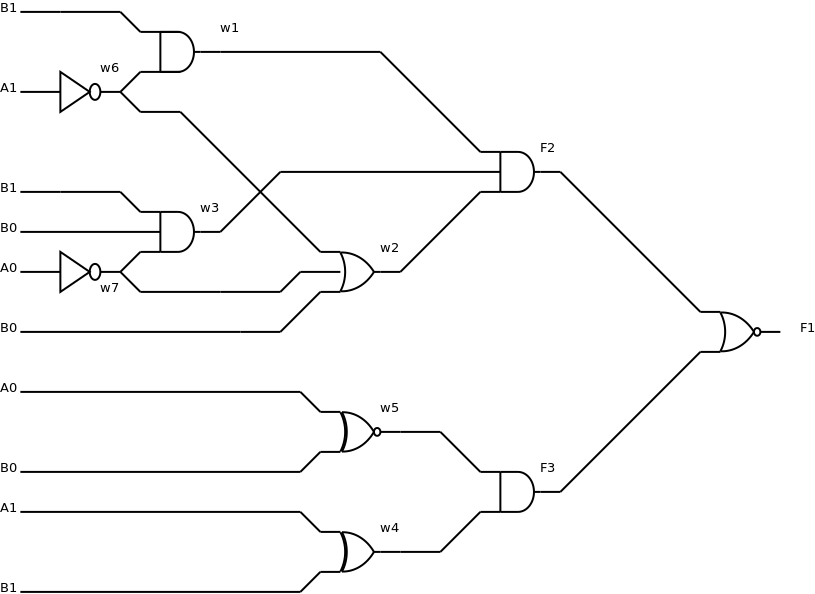
\includegraphics[width=.5\textwidth, center]{Diagram3.png}
\end{center}

\hfill
\item[\textbf{\en{iiic.}}]
\hfill
\begin{center}
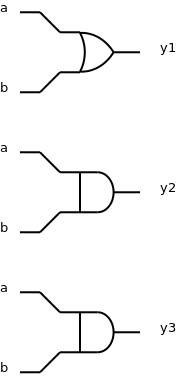
\includegraphics[width=.15\textwidth, center]{Diagram4.png}
\end{center}
\end{enumerate}
